% Matlab.tex
%
% Notes:
%
% o Rename this file appropriately.
%
% o Complete relevant sections below.
%
% o Use markup commands defined in scirun-doc.sty.
%   Avoid presentation markup (e.g. \textbf or \emph).
%
% o To make your document web-friendly, use commands from html package. See
%   latex2html manual or the book "The Latex Web Companion."
%
% o Don't add new subsections, but freely subsubsection 
%   existing subsections.
%
% o Add local commands if desired (via \newcommand).  But first check for
%   equivalent markup in scirun-doc.sty.
%
% o Only use packages distributed with Latex2e.
%
% o Cite references with the \cite command. Put citations in
%   a bib file and send along with this file.
%
% o Please include at least one image of tk GUI. Provide 
%   an EPS version and a web friendly version (e.g., jpeg or gif).
%
% o Including images:  Create a figure command for each figure using   the
%   template below.  Copy the template (make a copy of the template
%   for each figure) and uncomment only the first '%' in each line.
%   Then replace bracketed text with appropriate values.  Here is  the
%   template: 
%%begin{latexonly}
%  \newcommand{\<figure command name>}%
%  {\centerline{\includegraphics[options]{<path to eps file>}}}
%%end{latexonly}
%\begin{htmlonly}
%  \newcommand{\<figure command name (same as above)>}{%
%  \htmladdimg[options]{<path to jpg file>}}
%\end{htmlonly}
%
%   Where in the ``latexonly'' part, ``options'' is a list of key-value pair
%   options.  Typically the options specify graphic width, height, and
%   bounding box.  See ``The Latex Graphics Companion'' for more
%   information.  Note that we are using ``\includegraphics'' command
%   from the ``graphicx'' package.
%
%   In the ``htmlonly'' part ``options'' is a list options such as ``align'',
%   ``width'', ``height'', and ``alt''.  See ``The Latex Web Companion'' for
%   details.
%   
%   Now to actually create figures enclose each figure command as follows:
%
%\begin{figure}
%  \begin{makeimage}
%  \end{makeimage}
%  \<figurecommand>
%  \caption{\label{fig:<figure label>} <Caption text>}
%\end{figure}
%
%   and replace bracket text appropriately.
%   
%%%%%%%%%%%%%%%%%%%%%%%%%%%%%%%%%%%%%%%%%%%%%%%%%%%%%%%%%%%%%%%%%%%%%%

\newcommand{\mlm}{\module{Matlab module}}
\newcommand{\m}{\emph{Matlab}}

%%%% Images used in this file

%begin{latexonly}
  \newcommand{\tstone}%
  {\centerline{\includegraphics[width=4.5in]{figs/tst1.ps}}}
%end{latexonly}
\begin{htmlonly}
  \newcommand{\tstone}{%
  \htmladdimg[]{../figs/tst1.jpg}}
\end{htmlonly}

%begin{latexonly}
  \newcommand{\tsttwo}%
  {\centerline{\includegraphics[width=4.5in]{figs/tst2.ps}}}
%end{latexonly}
\begin{htmlonly}
  \newcommand{\tsttwo}{%
  \htmladdimg[]{../figs/tst2.jpg}}
\end{htmlonly}

%begin{latexonly}
  \newcommand{\tstthree}%
  {\centerline{\includegraphics[width=4.5in]{figs/tst3.ps}}}
%end{latexonly}
\begin{htmlonly}
  \newcommand{\tstthree}{%
  \htmladdimg[]{../figs/tst3.jpg}}
\end{htmlonly}

%%%%%%%%%%%%%%%%%%%%%%%%%%%%%%%%%%%%%%%%%%%%%%%%%%%%%%%%%%%%%%%%%%%%%%
\ModuleRef{\Module{Matlab}}{\Category{DataIO}}{\Package{MatlabInterface}}

\subsection{Summary} 

The \mlm{} is part of the \Package{MatlabInterface} package that enables
calls from \sr{} to \m{}, either to interactive commands or via \m{}
scripts.  Sockets are the underlying coupling mechanism that connect \sr{}
and m{} because they run as separate processes.  The \mlm{} facilitates
both simple tasks such as converting files between \sr{} and \m{}, and more
complex tasks such as creating interactive \sr{} programs that call \m{}
scripts to perform real-time applications.

\subsection{Use}

The following five examples of the \package{MatlabInterface} package
demonstrate how to work with the \mlm{}.  The first three examples,
\filename{tst1.net}, \filename{tst2.net}, and \filename{tst3.net}, assume
that \sr{} and \m{} reside on the same host, while the fourth example
\filename{tst4.net}, illustrates the case in which \sr{} and \m{} reside on
different hosts. The fifth example, \filename{tst5.net}, demonstrates how
to apply the \mlm{} to an example of complex \m{} code: the focusing
inversion routine.

\subsubsection{Example 1: Saving the Matlab matrix in \sr{} format} 


To execute the first example, begin from your Unix shell and change to the
directory that contains the networks and data files:
%
\begin{verbatim}
cd $SCIRun/src/Packages/MatlabInterface/matlab/engine
\end{verbatim}
%
The \variable{SCIRun} identifies the top level directory of your 
local
\sr{} source code tree.

Now, launch \sr{} with the name of the first test net as the 
argument 
%
\begin{verbatim}
$SCIRun/bin/scirun  tst1.net
\end{verbatim}

Executing the net will cause \m{} to generate a random matrix and sends it
to \sr{}, which will save the contents as a \sr{} file.  Your screen should
be similar to the contents of Figure \ref{fig:tst1}.


\begin{figure}[htb]
  \begin{makeimage}
  \end{makeimage}
  \tstone
  \caption{\label{fig:tst1} Screen capture for the first test
  example.}
\end{figure}


In Figure \ref{fig:tst1}, the uppermost window shows the \sr{} environment,
while the Unix terminal appears in the lowermost window (with a black
background, titled "rapture," indicating where the package started).  Any
diagnostic output will appear in the Unix terminal window.

The "GUI dialog window" is the white window labeled "Matlab\_O," visible in
Figure \ref{fig:tst1}. Any commands entered in this window pass to \m{} for
execution. In this example,
%
\begin{verbatim}
o1=rand(5,5);
\end{verbatim}
%
instructs \m{} to generate a 5~$\times$~5 matrix of random numbers.

The line containing \variable{host:port} that appears at the top of the
\mlm{} GUI dialog window below the title ``Matlab\_O,'' contains the
network address (IP address and port) of the computer running the \m{}
engine.  Because \m{} and \sr{} operate on the same computer, the IP
address is the local loopback, \ipaddr{127.0.0.1}, and the port is
\port{5517}. We recommend that ports have numbers above \port{5000} and any
value in this range is acceptable (\ie{} not reserved by the operating
system).

Note that the use of address \ipaddr{127.0.0.1} not only signifies the fact
that \sr{} and \m{} will run on the same computer, but also instructs
\mlm{} to start the \m engine automatically in the background (\ie{}
without user interference).  If you wish to use \sr and \m{} on the same
machine, but run \m{} manually (such as described in in Example 4), use the
address \ipaddr{localhost}.

Following the host and IP address, the \variable{host:port} line also
contains the debug \variable{wordy} parameter, an integer that controls the
verbosity of the diagnostic output.  A \variable{wordy} parameter of 0
indicates no output, 1 indicates little output, whereas 5 indicates a very
verbose output.

In Figure \ref{fig:tst1}, the \mlm{} appears to the left of the GUI dialog
window.  This module has five matrix-type input and output ports colored in
light blue.  In the \mlm{} GUI dialog window, the input ports have mnemoic
names referenced as: \variable{i1}, \variable{i2}, ariable{i3},
\variable{i4}, and \variable{i5}.  The five output ports are named
\variable{o1}, \variable{o2}, \variable{o3}, \variable{o4}, and
\variable{o5}.

This example uses only the output port, \variable{o1}, to send the
random matrix to \sr{}, which, in turn, saves it in a file.

Executing the \mlm{}, by pressing the ``Execute'' button on the bottom of
the GUI dialog window, initiates the following sequence:
%
\begin{enumerate}
  \item The \mlm{} automatically launches \m{} with the engine script in
        the background. 
  \item If necessary, the engine compiles any necessary components.
  \item The engine starts listening at \socket{127.0.0.1}{5517}.
  \item \mlm{} sends the command in the GUI dialog window to the engine
        via the socket.
  \item The engine receives and executes the command, creating
        variable \variable{o1}.
  \item \m{} sends the variable
        \variable{o1} back to \sr{} via the socket.
  \item The  \mlm{} receives the matrix and sends it downstream to
        the \module{MatrixWriter} module. 
  \item \module{MatrixWriter} saves the matrix to disk as the
        \filename{rand1.mat} file. 
\end{enumerate}

You may shut down the \m{} engine from the \mlm{} GUI dialog window by
pressing your left mouse button, and choosing destroy (this will destroy
the \mlm{}).

To determine whether you ran this example properly, you may open the file
\filename{rand1.mat } with any ASCII text editor. The file should contain a
random $5 \times 5$ matrix in \sr{} format.

\subsubsection{Example 2: Converting a \sr{} file to a raw
ASCII \m{} file}  

The second example runs with the \filename{tst2.net} file, which you will
find in the same directory as for the previous example:
%
\begin{verbatim}
$SCIRun/src/Packages/MatlabInterface/matlab/engine
\end{verbatim}

Now, start \sr{} again with {\bf tst2.net} as the command line
argument: 
%
\begin{verbatim}
$SCIRun/bin/scirun  tst2.net
\end{verbatim}
%
Your window should be similar to that in the image in Figure
\ref{fig:tst2}.

\begin{figure}[htb]
  \begin{makeimage}
  \end{makeimage}
  \tsttwo
  \caption{\label{fig:tst2} Screen capture for the second test
  example. This test example reads a
  file from the disk in \sr{} format and saves it in \m{} format.}
\end{figure}

This net uses the \module{MatrixReader} module to read a file in \sr{}
format (\filename{rand1.mat}), and then passes the contents to \m{}.  \m{}
saves the contents in ASCII format as \filename{rand2.mat} by executing the
command the appears in the \mlm{} GUI dialogue window of Figure
\ref{fig:tst2}:
%
\begin{verbatim}
save -ascii rand2.dat i1
\end{verbatim} 

In the \mlm{} GUI dialog window, you may press the``Execute'' button to
initiate the following sequence:
%
\begin{enumerate}
  \item \module{MatrixReader} reads \filename{rand1.mat} from disk.
  \item The \mlm{} fires, accepting the matrix on the first port.
  \item \m{} automatically runs with the engine script in the background.
  \item The engine starts listening at \socket{127.0.0.1}{5517}.
  \item The \mlm{} sends the matrix to the engine, creating the \variable{i1}
        variable. 
  \item The \mlm{} sends the save command to the engine via the
        socket. 
  \item The engine receives and executes the command, saving the matrix to
        the file \filename{rand2.dat}. 
\end{enumerate}

To finish the script, shut down the \mlm{} as described above.

You may determine whether this example ran properly by opening the file
\filename{rand2.dat}, which should contain the same random numbers as the
file \filename{rand1.mat}.

\subsubsection{Example 3: Converting a \m{} file to a \sr{} file} 

The third \mlm{} example runs with the \filename{tst3.net} file in the
directory:
%
\begin{verbatim}
$SCIRun/src/Packages/MatlabInterface/matlab/engine
\end{verbatim}

To initiate this example, start \sr{} again with \filename{tst3.net} 
as the
command line argument:
%
\begin{verbatim}
$SCIRun/bin/scirun  tst3.net
\end{verbatim}

\begin{figure}[htb]
  \begin{makeimage}
  \end{makeimage}
  \tstthree
  \caption{\label{fig:tst3} Screen capture for the third test 
example. This
  example reads a \m{} file, and saves it in \sr{} format. }
\end{figure}

Figure \ref{fig:tst3} shows the resulting screen view for this example. The
net reads the \m{} file \filename{rand2.dat} from disk and sends it to
\sr{}, then saves it as the \filename{rand3.mat} file in \sr{} ASCII
format.

The command in the \mlm{} GUI dialog window this time is:
%
\begin{verbatim}
o1=load('rand2.dat'),
\end{verbatim}
and the module uses only one output port, \variable{o1}. 

In the \mlm{} GUI dialog window, press the "Execute" button to initiate the
following sequence:
%
\begin{enumerate}
  \item The \mlm{} automatically runs \m{} with the engine script in 
        the background. 
  \item The engine starts listening at \socket{127.0.0.1}{5517}.
  \item The \mlm{} sends the command \icode{o1=load('rand2.dat')} 
        command
        to the engine via the socket.   
  \item The engine receives and executes the command, creating the 
        variable
        \variable{o1}.
  \item The \mlm{} sends the variable \variable{o1} back to \sr{} 
        via the
        socket. 
  \item The \mlm{} receives the matrix and sends it
        downstream to the \module{MatrixWriter} module, which saves
        it as the \sr{} file \filename{rand3.mat}.
\end{enumerate}

To finish this example, shut down the \mlm{} as in previous 
examples.

You may determine whether this example ran properly by opening the file
\filename{rand3.mat}, which should contain the same random numbers as files
\filename{rand1.mat}, and \filename{rand2.dat}.

\subsubsection{ \sr{} and \m{} on different hosts}  

The network for this example is the same as that in the first example,
however, it will execute in a different condition. Here, we assume that \m{}
and \sr{} run on different hosts and so must pass information and data
across the network between the two computers.  We also assume that \m{}
runs on the host \ipaddr{burn.cs.utah.edu} (or \ipaddr{burn}) and \sr{} on
the host \ipaddr{rapture.sci.utah.edu}, or \ipaddr{rapture}].

In this case, only the contents of the directory: 
%
\begin{verbatim}
$SCIRun/src/Packages/MatlabInterface
\end{verbatim}
%
need be available on \ipaddr{burn}; the rest of the \sr{} source tree must
only be available on \ipaddr{rapture} because we assume this host to be
running \sr{}.

From within the directory on \ipaddr{burn}, launch \m{} and then run the
\filename{mlabengine.m} script with the second argument set to
\ipaddr{rapture}:
%
\begin{verbatim}
mlabengine(0,'rapture.sci.utah.edu:5515')
\end{verbatim}
%
\m{} now runs on \ipaddr{burn} and is ready to accept remote commands from
our second host, in this case, \ipaddr{rapture}.

Assuming that \sr{} runs on \ipaddr{rapture}, carry out the
following steps:
%
\begin {enumerate}
  \item Download the script \filename{tst1.net} 
        into the \sr{} directory on \ipaddr{rapture}. 
  \item Launch \sr{} as described above with the \filename{tst1.net} 
        net,
  \item Before executing the \mlm{}, edit the \variable{host:port} 
        string to be \socket{burn.cs.utah.edu:5515} (Note: the port address
        must agree with the one specified in the \icode{mlabengine} command
        above).
  \item Execute the network by pressing the ``Execute'' button at 
        the bottom of the \mlm{} GUI dialog window, which will save the
        random matrix $5\times 5$, as it did in the first example.  This
        time, the data for this file has come from \ipaddr{burn}, to be
        saved on \ipaddr{rapture}.
\end{enumerate}

The actual sequence of events is as follows:
%
\begin{enumerate}
  \item The \mlm{} executes on \ipaddr{rapture}, sending the \m{} 
        command
        to the engine on \ipaddr{burn} via the socket,
  \item The engine receives and executes the command on 
        \ipaddr{burn} and creates the variable \variable{o1},
  \item \ipaddr{burn} sends the variable  variable{o1} back to \sr{} on
        \ipaddr{rapture} via the socket,
  \item On \ipaddr{rapture}, the \mlm{} receives the matrix and 
        sends it downstream to the \module{MatrixWriter} module,
  \item \module{MatrixWriter} saves the matrix to disk as the file
        \filename{rand1.mat}.
\end{enumerate}

Terminating this example requires operations on both hosts:
%
\begin{enumerate} 
  \item On \ipaddr{rapture}, quit \sr{}.  
  \item On \ipaddr{burn}, press {\bf control-C} to terminate the
        \command{mlabengine.m} script.
  \item Quit \m{}.
\end{enumerate}

\subsubsection{Example 5: Focusing inversion} 


In this final example, focusing inversion provides a special solution to
the inverse problem
%
\begin{equation}
  \mathbf{F} \mathbf{m} = \mathbf{d} 
\end{equation}
%
where we solve for the vector $\mathbf{m}$, given an ill-conditioned
transform matrix $\mathbf{F}$ and a right hand side $\mathbf{d}$.  We
assume this problem is essentially underdetermined and hence that matrix
${\bf F}$ is rectangular.

In this example, the algorithm receives matrix $\mathbf{F}$ and vector
$\mathbf{d}$ as input, and returns the solution as a vector $\mathbf{m}$.

The files required for this example reside in the directory:
%
\begin{verbatim}
$SCIRun/src/Packages/MatlabInterface/matlab/fcs
\end{verbatim}

In the first part of this example, we prepare a random sample matrix,
$\mathbf{F}$ and a vector, $\mathbf{d}$.  Then we pass these to the
associated \m{} program that computes the solution to the inverse
problem for those input variables.

To carry out this example:
%
\begin{enumerate}
  \item Change your working directory to
        \begin{verbatim}
        $SCIRun/src/Packages/MatlabInterface/matlab/fcs
        \end{verbatim}  
  \item Edit the script \filename{scirun.bat}, which refers to an
        executable version of \sr{} available on your system.
  \item Launch \sr{} by executing the command:\\
        \begin{verbatim}
        scirun.bat prepare.net
        \end{verbatim} 
        Executing the net will produce files \filename{f.mat} 
        and \filename{dd.mat} (sensitivity and data matrices).
  \item Manually destroy the \mlm{} to shut down \m{}.
  \item Quit \sr{}.
\end{enumerate}

We now have the matrix $\mathbf{F}$ stored in the file \filename{f.mat},
and the data vector $\mathbf{d}$ stored in the file \filename{dd.mat}
in ASCII format.  $\mathbf{F}$ is the 100*900 random matrix, and
$\mathbf{d}$ is a vector containing 100 values.

Focusing inversion accepts these data as input, calls a \m{} script
\filename{fcs.m} to produce the solution, and saves the solution into the
file \filename{res.mat}.

In order to run focusing:
%
\begin{enumerate}
  \item Launch \sr{} again with the command:
        \begin{verbatim}
        scirun.bat fcs.net
        \end{verbatim}
        and run the net. This will produce the file 
\filename{res.mat}
        (a result of the focusing inversion)
  \item Manually destroy the \mlm{} to shut down \m{}. 
  \item Quit \sr{}.
\end{enumerate}

The resulting file, \filename{res.mat}, should contain a vector of
900 values that is the solution to the inversion.

\subsection{Details}

We have already demonstrated that \sr{} communicates with \m{} via network
sockets.  Communication overhead is minimal when both packages reside on
the same machine, and increases (depending on the network speed) when \m{}
runs from a remote host.

The network communication model allows remote calls to \m{} scripts and
also uses \m{} as a scripting engine to process interactive user
requests. We chose the network communication model over other options
because of its greater flexibility. This model also resolves potential
licensing conflicts and provides convenience by potentially saving extra
installation time when \sr{} and \m{} already exist on different hosts.


\subsection{Notes}

\subsubsection{Location and installation}

We assume the environment variable \envvar{SCIRun} points to the root of
the \sr{} source tree, and that the package executables are available in
the directory \directory{SCIRun/bin}.

To install the \mlm{} package, at configure time, provide the following
option to the configure script:
%
\begin{verbatim}
configure --with-package=MatlabInterface,
\end{verbatim}
%
and run \command{gmake } in the \directory{SCIRun/bin} directory.

The example \m{} engine networks and scripts (\filename{tst*.net} files)
are located in the \sr{} source tree under\\
\directory{\$SCIRun/src/Packages/MatlabInterface/matlab/engine}.

\subsubsection{Bugs}

\m{} graphics do not work under the current version of the \mlm{}.  If the
script contains graphics commands (\eg{} ``plot''), the \m{} graphics
window does not appear and may produce an error.

\subsection{Credits} 

The \mlm{} was written by Oleg Portniaguine with help from Marty Cole,
David Weinstein and Michael Callahan.  Robert MacLeod, Steve Parker and
Yesim Serinagaoglu also provided useful suggestions.

